\documentclass[dvipdfmx]{jsarticle}


\usepackage{tcolorbox}
\usepackage{color}
\usepackage{listings, plistings}

%% ノート/latexメモ
%% http://pepper.is.sci.toho-u.ac.jp/pepper/index.php?%A5%CE%A1%BC%A5%C8%2Flatex%A5%E1%A5%E2

%% JavaScriptの設定
%% https://e8l.hatenablog.com/entry/2015/11/29/232800
\lstdefinelanguage{javascript}{
  morekeywords = [1]{ %keywords
    await, break, case, catch, class, const, continue, debugger, default, delete, 
    do, else, enum, export, extends, finally, for, function, function*, if, implements, import, in, 
    instanceof, interface, let, new, package, private, protected, public, return, static, super,
    switch, this, throw, try, typeof, var, void, while, with, yield, yield*
  },
  morekeywords = [2]{ %literal
    false, Infinity, NaN, null, true, undefined
  },
  morekeywords = [3] { %Classes
    Array, ArrayBuffer, Boolean, DataView, Date, Error, EvalError, Float32Array, Float64Array,
    Function, Generator, GeneratorFunction, Int16Array, Int32Array, Int8Array, InternalError,
    JSON, Map, Math, Number, Object, Promise, Proxy, RangeError, ReferenceError, Reflect,
    RegExp, Set, String, Symbol, SyntaxError, TypeError, URIError, Uint16Array, Uint32Array,
    Uint8Array, Uint8ClampedArray, WeakMap, WeakSet
  },
  morecomment = [l]{//},
  morecomment = [s]{/*}{*/},
  morestring = [b]{"},
  morestring = [b]{'},
  alsodigit = {-},
  sensitive = true
}

%% 修正時刻: Tue 2022/03/15 10:04:41


% Java
\lstset{% 
  frame=single,
  backgroundcolor={\color[gray]{.9}},
  stringstyle={\ttfamily \color[rgb]{0,0,1}},
  commentstyle={\itshape \color[cmyk]{1,0,1,0}},
  identifierstyle={\ttfamily}, 
  keywordstyle={\ttfamily \color[cmyk]{0,1,0,0}},
  basicstyle={\ttfamily},
  breaklines=true,
  xleftmargin=0zw,
  xrightmargin=0zw,
  framerule=.2pt,
  columns=[l]{fullflexible},
  numbers=left,
  stepnumber=1,
  numberstyle={\scriptsize},
  numbersep=1em,
  language={Java},
  lineskip=-0.5zw,
  morecomment={[s][{\color[cmyk]{1,0,0,0}}]{/**}{*/}},
  keepspaces=true,         % 空白の連続をそのままで
  showstringspaces=false,  % 空白字をOFF
}
%\usepackage[dvipdfmx]{graphicx}
\usepackage{url}
\usepackage[dvipdfmx]{hyperref}
\usepackage{amsmath, amssymb}
\usepackage{itembkbx}
\usepackage{eclbkbox}	% required for `\breakbox' (yatex added)
\usepackage{enumerate}
\usepackage[default]{cantarell}
\usepackage[T1]{fontenc}
\fboxrule=0.5pt
\parindent=1em
\definecolor{mygrey}{rgb}{0.97, 0.97, 0.97}

\makeatletter
\def\verbatim@font{\normalfont
\let\do\do@noligs
\verbatim@nolig@list}
\makeatother

\begin{document}

%\anaumeと入力すると穴埋め解答欄が作れるようにしてる。\anaumesmallで小さめの穴埋めになる。
\newcounter{mycounter} % カウンターを作る
\setcounter{mycounter}{0} % カウンターを初期化
\newcommand{\anaume}[1][]{\refstepcounter{mycounter}{#1}{\boxed{\phantom{aa}\textnormal{\themycounter}\phantom{aa}}}} %穴埋め問題の空欄作ってる。
\newcommand{\anaumesmall}[1][]{\refstepcounter{mycounter}{#1}{\boxed{\tiny{\phantom{a}\themycounter \phantom{a}}}}}%小さい版作ってる。色々改造できる。

%% 修正時刻: Tue 2022/03/15 10:04:411


\section{MySQL その他}

以下は、MySQLがどんな設定で動作しているかということで、
特に指定しなくても困らない。

\subsection{文字コードあるいは文字セット}

単に文字コードといった場合、文字セットを指すことが多い。

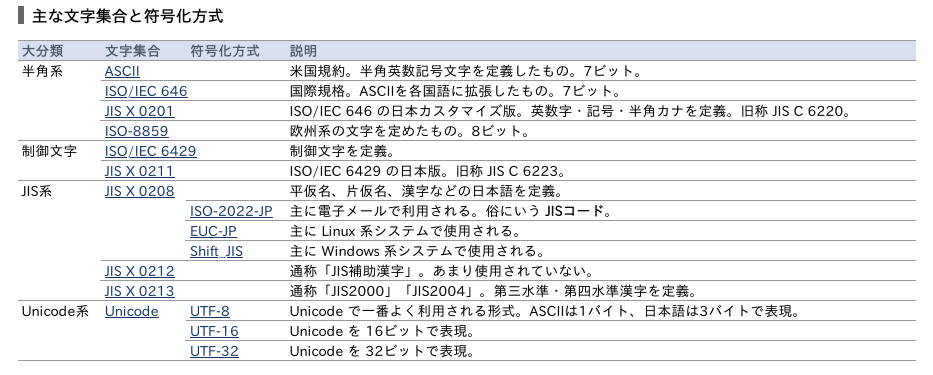
\includegraphics[width=15cm]{../06-mysql/character-set.png} \\
\rightline{\href{https://www.tohoho-web.com/ex/charset.html}
{(出典)文字コード入門 https://www.tohoho-web.com/ex/charset.html}}



\subsubsection{MySQLの文字コード(文字セット)}

MySQLにログインする。

\begin{tcolorbox}
 $>$ mysql -u sampleuser -p \\
 Enter password: ********
 MariaDB [(none)]$>$
\end{tcolorbox}

ここで以下のコマンドを実行する。

\begin{tcolorbox}
 MariaDB [(none)]$>$ show variables like \verb!'%char%'!;
\end{tcolorbox}
\rightline{※ これは ``'char'という文字列を\underline{含む}変数を表示しなさい'' と
いう意味のコマンドである。}

\begin{spacing}{0.8}
\begin{verbatim}
+--------------------------+--------------------------------+
| Variable_name            | Value                          |
+--------------------------+--------------------------------+
| character_set_client     | cp932                          |
| character_set_connection | cp932                          |
| character_set_database   | utf8mb4                        |
| character_set_filesystem | binary                         |
| character_set_results    | cp932                          |
| character_set_server     | utf8mb4                        |
| character_set_system     | utf8                           |
| character_sets_dir       | C:\xampp\mysql\share\charsets\ |
+--------------------------+--------------------------------+
\end{verbatim}
\end{spacing}

MySQL は、サーバープログラムとクライアントプログラムで動作している。

XAMPPコントロールパネルで ``Start'' ボタンをクリックしがのは、
サーバープログラムを起動しているのである。

コマンドプロンプトで ``mysql -u sampleuser -p'' としているのは、
クライアントプログラムを使って、サーバープログラムに接続し、
ログイン処理をおこなっているのである。

普通はサーバーはネットワーク上のどこか離れた場所にあるのだけれど、
XAMPPでは、各自のパソコン内でサーバープログラムと
クライアントプログラムが動いていることになる。

さて、上記の結果の意味は以下である。

\begin{tcolorbox}
\begin{tabular}{lcl} 
character\_set\_client     & : & cp932 \\
\end{tabular}

\hspace{8mm}クライアントの文字セットは cp932(SJIS)である。

\begin{tabular}{lcl} 
character\_set\_connection & : & cp932 \\
\end{tabular}

\hspace{8mm}クライアントから受け取った文字を cp932(SJIS)に変換する。
 
\begin{tabular}{lcl} 
character\_set\_database   & : & utf8mb4 \\
\end{tabular}

\hspace{8mm}データベースで使用する文字セットは utf8mb4 である。
 
\begin{tabular}{lcl} 
character\_set\_filesystem & : & binary  \\
\end{tabular}


\begin{tabular}{lcl} 
character\_set\_results    & : & cp932   \\
\end{tabular}

\hspace{8mm}クライアントへ結果を送信するときの文字セットは cp932(SJIS) である。

\begin{tabular}{lcl} 
character\_set\_server     & : & utf8mb4 \\
\end{tabular}

\hspace{8mm}データベース作成時の既定の文字セット

\begin{tabular}{lcl} 
character\_set\_system     & : & utf8 \\
\end{tabular}

\hspace{8mm}ファイル名をこの文字コードで使う。

\begin{tabular}{lcl} 
character\_sets\_dir       & : &
     C:\yen xampp\yen mysql\yen share\yen charsets\yen \\ 
\end{tabular}

\hspace{8mm}文字セットを扱う上で必須となるファイルを配置しているディレクトリ
\end{tcolorbox}

XAMPPの場合、初期状態(この状態)で Windowsに最適な設定になっているはずである。

\begin{quote}
クライアント --- cp932(Shift\_JIS) \\
サーバー     --- UTF-8
\end{quote}


\subsubsection{データベース作成時の文字セット}

MySQLはデータベースを作成するとき、\textsf{utf8mb4} という文字セットを使っている。

以下のコマンドを実行することで確認できる。
MySQLにログインした状態で実行する。

\begin{tcolorbox}
 MariaDB [(none)]$>$ show create database sample;
\end{tcolorbox}

\begin{spacing}{0.8}
\begin{verbatim}
+----------+---------------------------------------------------------------------+
| Database | Create Database                                                     |
+----------+---------------------------------------------------------------------+
| sample2  | CREATE DATABASE `sample` /*!40100 DEFAULT CHARACTER SET utf8mb4 */ |
+----------+---------------------------------------------------------------------+
\end{verbatim}
\end{spacing}

utf8 には utf8mb3(3バイト) と utf8mb4(4バイト) がある。

たとえば ``吉'' の下が長い文字は utf8mb3 には含まれない。

MySQL で 単に ``utf8'' と指定した場合は ``utf8mb3'' が指定されたことになる。
これは歴史的な経緯でそうなったらしい。
ただ、これは近いうちに ``utf8mb4'' になるらしい。(MySQL8.0ではそうなっているという)。

今回は何も指定せずにデータベースを作成したが、
``utf8mb4'' が暗黙のうちに指定されている。

\subsubsection{テーブル作成時の文字セット}

テーブル作成時の文字セットは、MySQLにログインし、sampleデータベースの使用を宣言してのち、
以下のコマンドを実行することで確認できる。

\begin{tcolorbox}
 MariaDB [(none)]$>$ show create table emp;
\end{tcolorbox}


\begin{spacing}{0.8}
\begin{verbatim}
CREATE TABLE `emp` (
  `id` int(11) NOT NULL AUTO_INCREMENT,
  `name` varchar(20) NOT NULL,
  `age` int(11) NOT NULL,
  `birthday` year(4) NOT NULL,
  `dept_id` char(3) DEFAULT NULL,
  PRIMARY KEY (`id`),
  KEY `fk_dept_id` (`dept_id`),
  CONSTRAINT `fk_dept_id` FOREIGN KEY (`dept_id`) REFERENCES `dept` (`id`)
) ENGINE=InnoDB AUTO_INCREMENT=5 DEFAULT CHARSET=utf8mb4
\end{verbatim}
\end{spacing}

\fbox{DEFAULT CHARSET=utf8mb4} とあるので、``utf8mb4''が使われているのがわかる。


\subsection{照合順序(collation)}

照合順序(collation)というのは、文字データを並び変える場合、どういう順序で並び変えるかということである。たとえば、``は''と''ば''と''ぱ''の場合とかである。

MySQLではテーブルを作成したときに、何も指定しなければ、``\textsf{utf8mb4\_general\_ci}''
という照合順序が指定される。

これは、\verb!> show table status from sample;! というコマンドで確認できる。

``\textsf{utf8mb4\_general\_ci}'' というのは、大文字と小文字を区別しないという指定である。

``Tom'' と ``tom'' が区別されるとややこしいから、通常はこの区別しないという指定でよい。

\subsection{ストレージエンジン}

MySQLでは、ストレージエンジンとして ``InnoDB'' というのが使われている。

MySQL5.5から ``InnoDB'' がデフォルトのストレージエンジンとなった。
それ以前は、MyISAM というのが使われていた。

``InnoDB''の大きな特徴としては ``外部キー制約'' が使えるようになったことがあげられる。





\end{document}

%% 修正時刻: Sat May  2 15:10:04 2020


%% 修正時刻: Fri Aug 13 10:22:26 2021
